\section{Experimental Results \& Tests}
Using our implementation, TRE and scan\_for\_matches, we were able to do some benchmarking in order to compare performances.

For this a virtual machine is created, using Oracle VirtualBox\footnote{virtualbox.org}. The machine running the virtualbox is running Windows 8.1 Pro x64 of an SSD, with 8,00 GB RAM, an AMD FX 4300 Quad-Core Processor 3.80 GHz, of which 1 core and 4096MB RAM was given to the virtual machine, which would run Ubuntu 14.04.2 LTS 64 bit.

For the benchmarking some data was required:
\begin{figure}[h!]
\centering
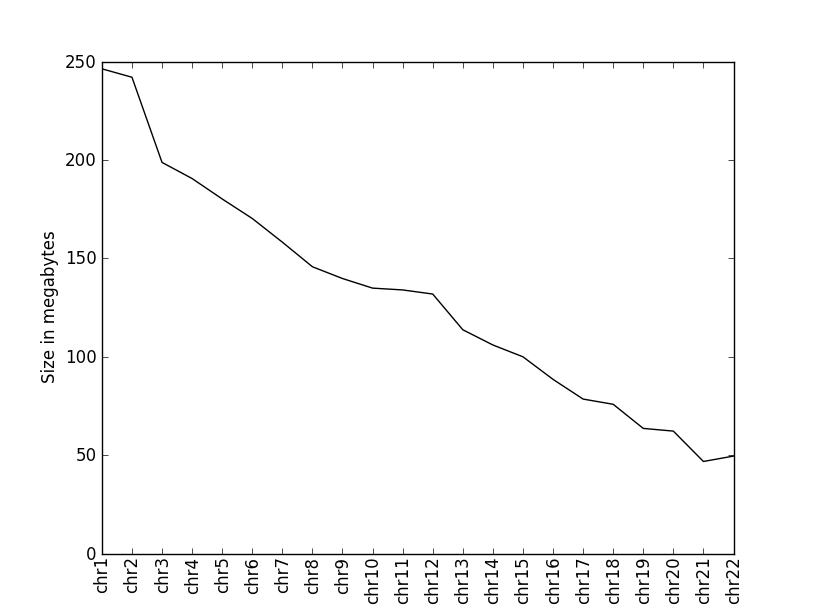
\includegraphics[width=0.5\textwidth]{Benchmarking/size.png}
\caption{Plot of sample files used for benchmarking, these files range from 246.3 Megabytes to 46.8 Megabytes in size}
\label{fig:size}
\end{figure}


Figure~\ref{fig:size} shows a series of fasta files, these files include nucleotide sequences, which all differ in size, decreasing from chr1 to chr22. These fasta files are the  kind of data which scan\_for\_matches are expected to run, and thus excellent for benchmark testing, it's worth noting however, that each of these files are 50 characters long, as TRE matches searches through lines separately, and longer or shorter line sizes might affect the performance of TRE, this was not tested.

For testing, a suitable pattern is required. As our implementation has primarily been focused on supporting insertion, deletion and mutation on a sequence, a simple RNA sequence $TGCAAGCGTTAAT$ with variable insertions is chosen as the search pattern.

Each test would be executed on each of the mentioned fasta files a total of 10 times, given an average runtime which was used in the following results.

First test using said sequence with 1 insertions:
\begin{figure}[h!]
\centering
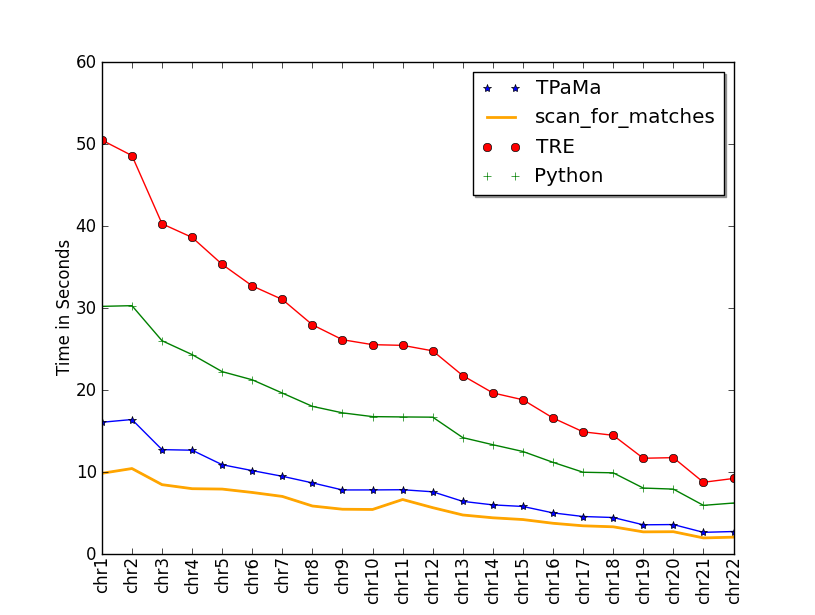
\includegraphics[width=0.5\textwidth]{Benchmarking/1ins.png}
\caption{Running time of search through fasta files mentioned in figure~\ref{fig:size},  allowing one insertions on pattern TGCAAGCGTTAAT}
\label{fig:ins1}
\end{figure}

From Figure~\ref{fig:ins1}, it's clear that given the 22 files, scan\_for\_matches runs faster than both our implementation, at roughly at half the time, and TRE which is about 5 times slower than scan\_for\_matches on this simple pattern.

Next test uses the same sequence but with two insertions instead of one.
\begin{figure}[h!]
\centering
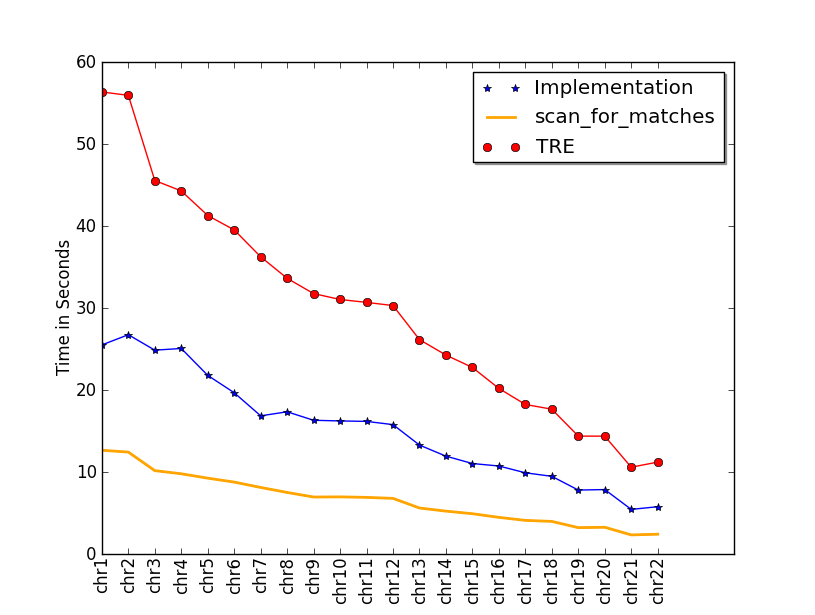
\includegraphics[width=0.5\textwidth]{Benchmarking/2ins.png}
\caption{Running time of search through fasta files mentioned in figure~\ref{fig:size},  allowing two insertions on pattern TGCAAGCGTTAAT}
\label{fig:ins2}
\end{figure}

While scan\_for\_matches did increase its runtime slightly, the second insertion really affected our implementation, resulting in it running at about the same speed as TRE.  And while TRE also had its runtime slightly increased, it's almost unchanged from one insertion.

Lastly there's three insertions:
\begin{figure}[h!]
\centering
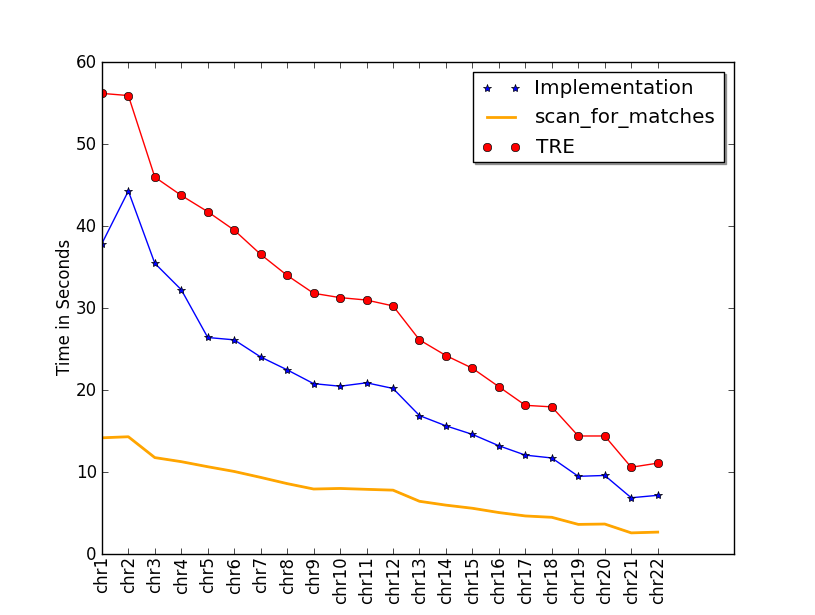
\includegraphics[width=0.5\textwidth]{Benchmarking/3ins.png}
\caption{Running time of search through fasta files mentioned in figure~\ref{fig:size},  allowing three insertions on pattern TGCAAGCGTTAAT}
\label{fig:ins3}
\end{figure}

In Figure~\ref{fig:ins3} our implementation really pulls away from scan\_for\_matches and TRE, which remains almost unchanged, relative to our implementation, which more than doubles its runtime.


From these three tests its clear to see that our implementation has a problem with increasing number of insertions, and as deletions and mutations are handled in a similar fashion we can conclude that our current implementation has a major flaw, should it be used with more advanced patterns. 
\\
~

Another interesting thing to test for was the number of hits when searching the files, in table~\ref{tab:hits} the number of hits which came up when searching on file chr1.fa are shown.

\begin{table}[h!]
\centering
\begin{tabular}{ l | c c r }
& 1 insertion & 2 insertions & 3 insertions\\
\hline
Our implementation& 5 &  47 & 235 \\
TRE& 1 & 19 & 76 \\
scan\_for\_matches & 5 & 43  & 192 \\
\end{tabular}
\caption{Number of hits in fasta file chr1, using the mentioned benchmark tests.}
\label{tab:hits}
\end{table}

The primary reason for our implementation to get more results than scan\_for\_matches is that our implementation finds every single match in the file, including overlapping matches, while scan\_for\_matches, by default, only finds matches which does not overlap. TRE has the major disadvantage here that it doesn't match across newlines, causing it to miss a lot of matches.

